% Options for packages loaded elsewhere
\PassOptionsToPackage{unicode}{hyperref}
\PassOptionsToPackage{hyphens}{url}
%
\documentclass[
]{article}
\usepackage{lmodern}
\usepackage{amssymb,amsmath}
\usepackage{ifxetex,ifluatex}
\ifnum 0\ifxetex 1\fi\ifluatex 1\fi=0 % if pdftex
  \usepackage[T1]{fontenc}
  \usepackage[utf8]{inputenc}
  \usepackage{textcomp} % provide euro and other symbols
\else % if luatex or xetex
  \usepackage{unicode-math}
  \defaultfontfeatures{Scale=MatchLowercase}
  \defaultfontfeatures[\rmfamily]{Ligatures=TeX,Scale=1}
\fi
% Use upquote if available, for straight quotes in verbatim environments
\IfFileExists{upquote.sty}{\usepackage{upquote}}{}
\IfFileExists{microtype.sty}{% use microtype if available
  \usepackage[]{microtype}
  \UseMicrotypeSet[protrusion]{basicmath} % disable protrusion for tt fonts
}{}
\makeatletter
\@ifundefined{KOMAClassName}{% if non-KOMA class
  \IfFileExists{parskip.sty}{%
    \usepackage{parskip}
  }{% else
    \setlength{\parindent}{0pt}
    \setlength{\parskip}{6pt plus 2pt minus 1pt}}
}{% if KOMA class
  \KOMAoptions{parskip=half}}
\makeatother
\usepackage{xcolor}
\IfFileExists{xurl.sty}{\usepackage{xurl}}{} % add URL line breaks if available
\IfFileExists{bookmark.sty}{\usepackage{bookmark}}{\usepackage{hyperref}}
\hypersetup{
  pdftitle={DS2 HW4},
  pdfauthor={Mufeng Xu},
  hidelinks,
  pdfcreator={LaTeX via pandoc}}
\urlstyle{same} % disable monospaced font for URLs
\usepackage[margin=1in]{geometry}
\usepackage{color}
\usepackage{fancyvrb}
\newcommand{\VerbBar}{|}
\newcommand{\VERB}{\Verb[commandchars=\\\{\}]}
\DefineVerbatimEnvironment{Highlighting}{Verbatim}{commandchars=\\\{\}}
% Add ',fontsize=\small' for more characters per line
\usepackage{framed}
\definecolor{shadecolor}{RGB}{248,248,248}
\newenvironment{Shaded}{\begin{snugshade}}{\end{snugshade}}
\newcommand{\AlertTok}[1]{\textcolor[rgb]{0.94,0.16,0.16}{#1}}
\newcommand{\AnnotationTok}[1]{\textcolor[rgb]{0.56,0.35,0.01}{\textbf{\textit{#1}}}}
\newcommand{\AttributeTok}[1]{\textcolor[rgb]{0.77,0.63,0.00}{#1}}
\newcommand{\BaseNTok}[1]{\textcolor[rgb]{0.00,0.00,0.81}{#1}}
\newcommand{\BuiltInTok}[1]{#1}
\newcommand{\CharTok}[1]{\textcolor[rgb]{0.31,0.60,0.02}{#1}}
\newcommand{\CommentTok}[1]{\textcolor[rgb]{0.56,0.35,0.01}{\textit{#1}}}
\newcommand{\CommentVarTok}[1]{\textcolor[rgb]{0.56,0.35,0.01}{\textbf{\textit{#1}}}}
\newcommand{\ConstantTok}[1]{\textcolor[rgb]{0.00,0.00,0.00}{#1}}
\newcommand{\ControlFlowTok}[1]{\textcolor[rgb]{0.13,0.29,0.53}{\textbf{#1}}}
\newcommand{\DataTypeTok}[1]{\textcolor[rgb]{0.13,0.29,0.53}{#1}}
\newcommand{\DecValTok}[1]{\textcolor[rgb]{0.00,0.00,0.81}{#1}}
\newcommand{\DocumentationTok}[1]{\textcolor[rgb]{0.56,0.35,0.01}{\textbf{\textit{#1}}}}
\newcommand{\ErrorTok}[1]{\textcolor[rgb]{0.64,0.00,0.00}{\textbf{#1}}}
\newcommand{\ExtensionTok}[1]{#1}
\newcommand{\FloatTok}[1]{\textcolor[rgb]{0.00,0.00,0.81}{#1}}
\newcommand{\FunctionTok}[1]{\textcolor[rgb]{0.00,0.00,0.00}{#1}}
\newcommand{\ImportTok}[1]{#1}
\newcommand{\InformationTok}[1]{\textcolor[rgb]{0.56,0.35,0.01}{\textbf{\textit{#1}}}}
\newcommand{\KeywordTok}[1]{\textcolor[rgb]{0.13,0.29,0.53}{\textbf{#1}}}
\newcommand{\NormalTok}[1]{#1}
\newcommand{\OperatorTok}[1]{\textcolor[rgb]{0.81,0.36,0.00}{\textbf{#1}}}
\newcommand{\OtherTok}[1]{\textcolor[rgb]{0.56,0.35,0.01}{#1}}
\newcommand{\PreprocessorTok}[1]{\textcolor[rgb]{0.56,0.35,0.01}{\textit{#1}}}
\newcommand{\RegionMarkerTok}[1]{#1}
\newcommand{\SpecialCharTok}[1]{\textcolor[rgb]{0.00,0.00,0.00}{#1}}
\newcommand{\SpecialStringTok}[1]{\textcolor[rgb]{0.31,0.60,0.02}{#1}}
\newcommand{\StringTok}[1]{\textcolor[rgb]{0.31,0.60,0.02}{#1}}
\newcommand{\VariableTok}[1]{\textcolor[rgb]{0.00,0.00,0.00}{#1}}
\newcommand{\VerbatimStringTok}[1]{\textcolor[rgb]{0.31,0.60,0.02}{#1}}
\newcommand{\WarningTok}[1]{\textcolor[rgb]{0.56,0.35,0.01}{\textbf{\textit{#1}}}}
\usepackage{graphicx}
\makeatletter
\def\maxwidth{\ifdim\Gin@nat@width>\linewidth\linewidth\else\Gin@nat@width\fi}
\def\maxheight{\ifdim\Gin@nat@height>\textheight\textheight\else\Gin@nat@height\fi}
\makeatother
% Scale images if necessary, so that they will not overflow the page
% margins by default, and it is still possible to overwrite the defaults
% using explicit options in \includegraphics[width, height, ...]{}
\setkeys{Gin}{width=\maxwidth,height=\maxheight,keepaspectratio}
% Set default figure placement to htbp
\makeatletter
\def\fps@figure{htbp}
\makeatother
\setlength{\emergencystretch}{3em} % prevent overfull lines
\providecommand{\tightlist}{%
  \setlength{\itemsep}{0pt}\setlength{\parskip}{0pt}}
\setcounter{secnumdepth}{-\maxdimen} % remove section numbering
\ifluatex
  \usepackage{selnolig}  % disable illegal ligatures
\fi

\title{DS2 HW4}
\author{Mufeng Xu}
\date{4/8/2021}

\begin{document}
\maketitle

\hypertarget{problem-1}{%
\section{Problem 1}\label{problem-1}}

\hypertarget{a.-regression-tree}{%
\subsection{A. Regression tree}\label{a.-regression-tree}}

\begin{Shaded}
\begin{Highlighting}[]
\FunctionTok{data}\NormalTok{(Prostate)}
\end{Highlighting}
\end{Shaded}

\hypertarget{the-lowest-cross-validation-error}{%
\subsubsection{The lowest cross-validation
error}\label{the-lowest-cross-validation-error}}

\begin{Shaded}
\begin{Highlighting}[]
\FunctionTok{set.seed}\NormalTok{(}\DecValTok{1}\NormalTok{)}

\NormalTok{ctrl }\OtherTok{=} \FunctionTok{trainControl}\NormalTok{(}\AttributeTok{method =} \StringTok{"cv"}\NormalTok{)}

\NormalTok{tree\_fit\_1 }\OtherTok{=} \FunctionTok{train}\NormalTok{(lpsa}\SpecialCharTok{\textasciitilde{}}\NormalTok{.,}
                   \AttributeTok{data =}\NormalTok{ Prostate,}
                   \AttributeTok{method =} \StringTok{"rpart"}\NormalTok{,}
                   \AttributeTok{tuneGrid =} \FunctionTok{data.frame}\NormalTok{(}\AttributeTok{cp =} \FunctionTok{exp}\NormalTok{(}\FunctionTok{seq}\NormalTok{(}\SpecialCharTok{{-}}\DecValTok{8}\NormalTok{,}\SpecialCharTok{{-}}\DecValTok{2}\NormalTok{, }\AttributeTok{length =} \DecValTok{20}\NormalTok{))),}
                   \AttributeTok{trControl =} \FunctionTok{trainControl}\NormalTok{(}\AttributeTok{method =} \StringTok{"cv"}\NormalTok{))}

\FunctionTok{ggplot}\NormalTok{(tree\_fit\_1, }\AttributeTok{highlight =} \ConstantTok{TRUE}\NormalTok{)}
\end{Highlighting}
\end{Shaded}

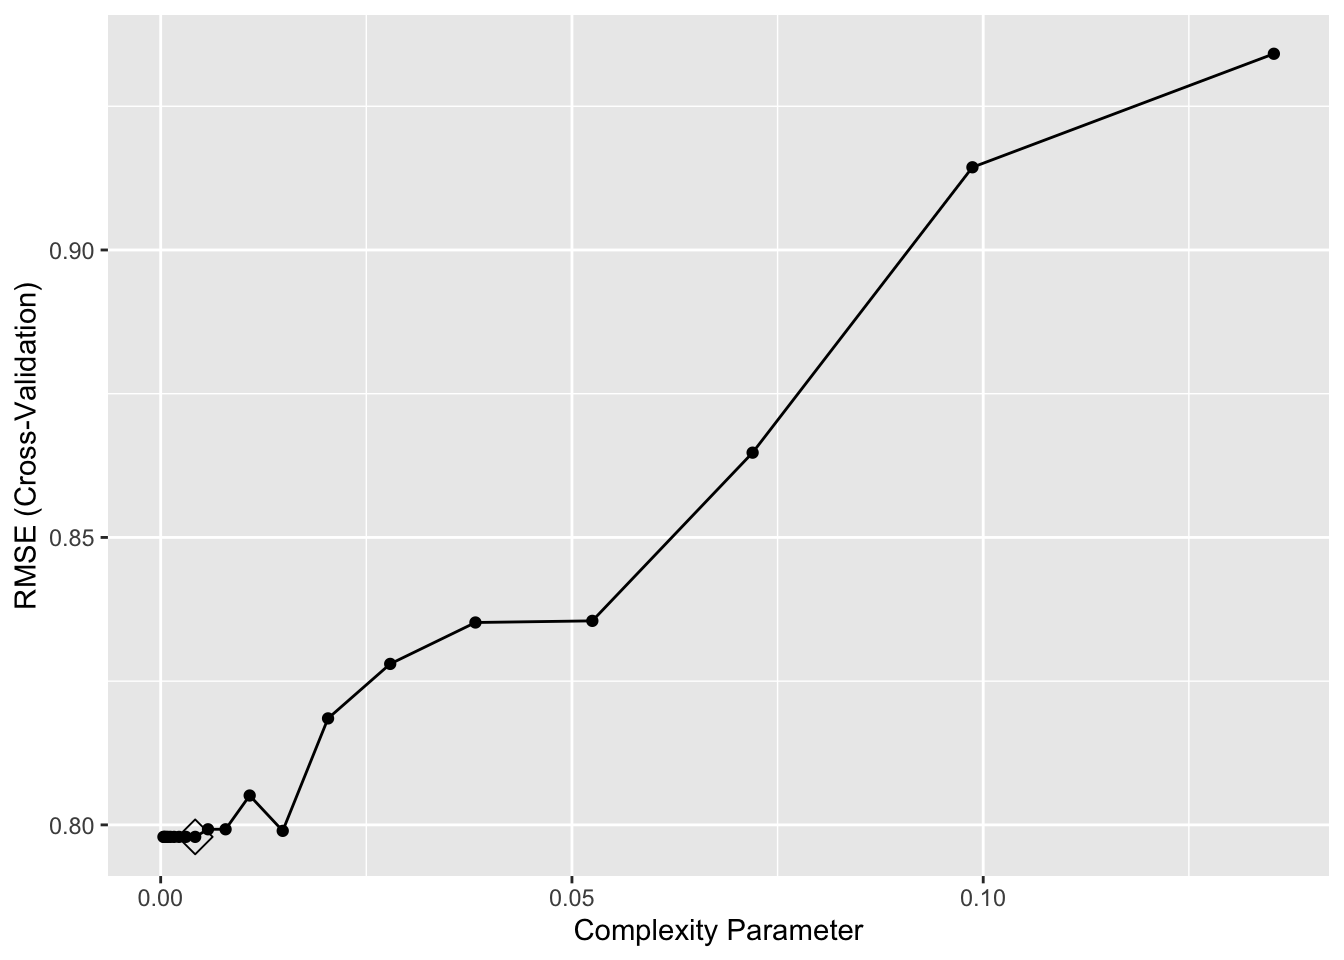
\includegraphics{hw4_files/figure-latex/unnamed-chunk-2-1.pdf}

\begin{Shaded}
\begin{Highlighting}[]
\NormalTok{tree\_fit\_1}\SpecialCharTok{$}\NormalTok{bestTune}
\end{Highlighting}
\end{Shaded}

\begin{verbatim}
##            cp
## 9 0.004195746
\end{verbatim}

\begin{Shaded}
\begin{Highlighting}[]
\NormalTok{tree\_fit\_1}\SpecialCharTok{$}\NormalTok{finalModel}\SpecialCharTok{$}\NormalTok{cptable}
\end{Highlighting}
\end{Shaded}

\begin{verbatim}
##           CP nsplit rel error
## 1 0.34710828      0 1.0000000
## 2 0.18464743      1 0.6528917
## 3 0.05931585      2 0.4682443
## 4 0.03475635      3 0.4089284
## 5 0.03460901      4 0.3741721
## 6 0.02156368      5 0.3395631
## 7 0.02146995      6 0.3179994
## 8 0.00000000      7 0.2965295
\end{verbatim}

\begin{Shaded}
\begin{Highlighting}[]
\FunctionTok{rpart.plot}\NormalTok{(tree\_fit\_1}\SpecialCharTok{$}\NormalTok{finalModel)}
\end{Highlighting}
\end{Shaded}

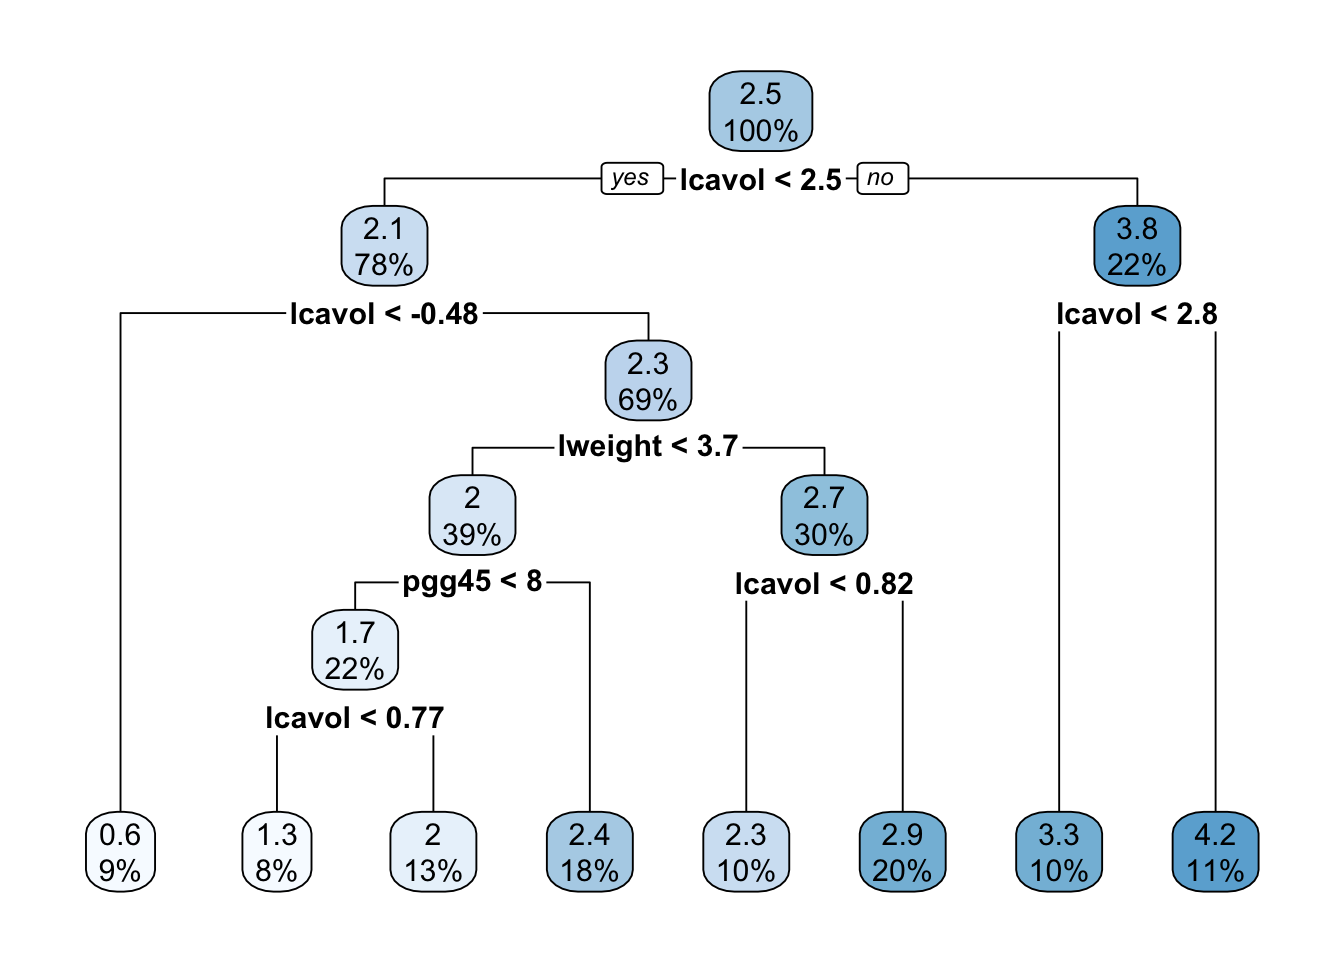
\includegraphics{hw4_files/figure-latex/unnamed-chunk-2-2.pdf}

\hypertarget{the-1-se-rule}{%
\subsubsection{The 1 SE rule}\label{the-1-se-rule}}

\begin{Shaded}
\begin{Highlighting}[]
\FunctionTok{set.seed}\NormalTok{(}\DecValTok{1}\NormalTok{) }
\NormalTok{tree\_fit\_2 }\OtherTok{=} \FunctionTok{train}\NormalTok{(lpsa}\SpecialCharTok{\textasciitilde{}}\NormalTok{.,}
                   \AttributeTok{data =}\NormalTok{ Prostate,}
                   \AttributeTok{method =} \StringTok{"rpart"}\NormalTok{,}
                   \AttributeTok{tuneGrid =} \FunctionTok{data.frame}\NormalTok{(}\AttributeTok{cp =} \FunctionTok{exp}\NormalTok{(}\FunctionTok{seq}\NormalTok{(}\SpecialCharTok{{-}}\DecValTok{8}\NormalTok{, }\SpecialCharTok{{-}}\DecValTok{2}\NormalTok{, }\AttributeTok{length =} \DecValTok{20}\NormalTok{))),}
                   \AttributeTok{trControl =} \FunctionTok{trainControl}\NormalTok{(}\AttributeTok{method =} \StringTok{"cv"}\NormalTok{,}
                                            \AttributeTok{number =} \DecValTok{10}\NormalTok{,}
                                            \AttributeTok{selectionFunction =} \StringTok{"oneSE"}\NormalTok{))}

\FunctionTok{ggplot}\NormalTok{(tree\_fit\_2, }\AttributeTok{highlight =} \ConstantTok{TRUE}\NormalTok{)}
\end{Highlighting}
\end{Shaded}

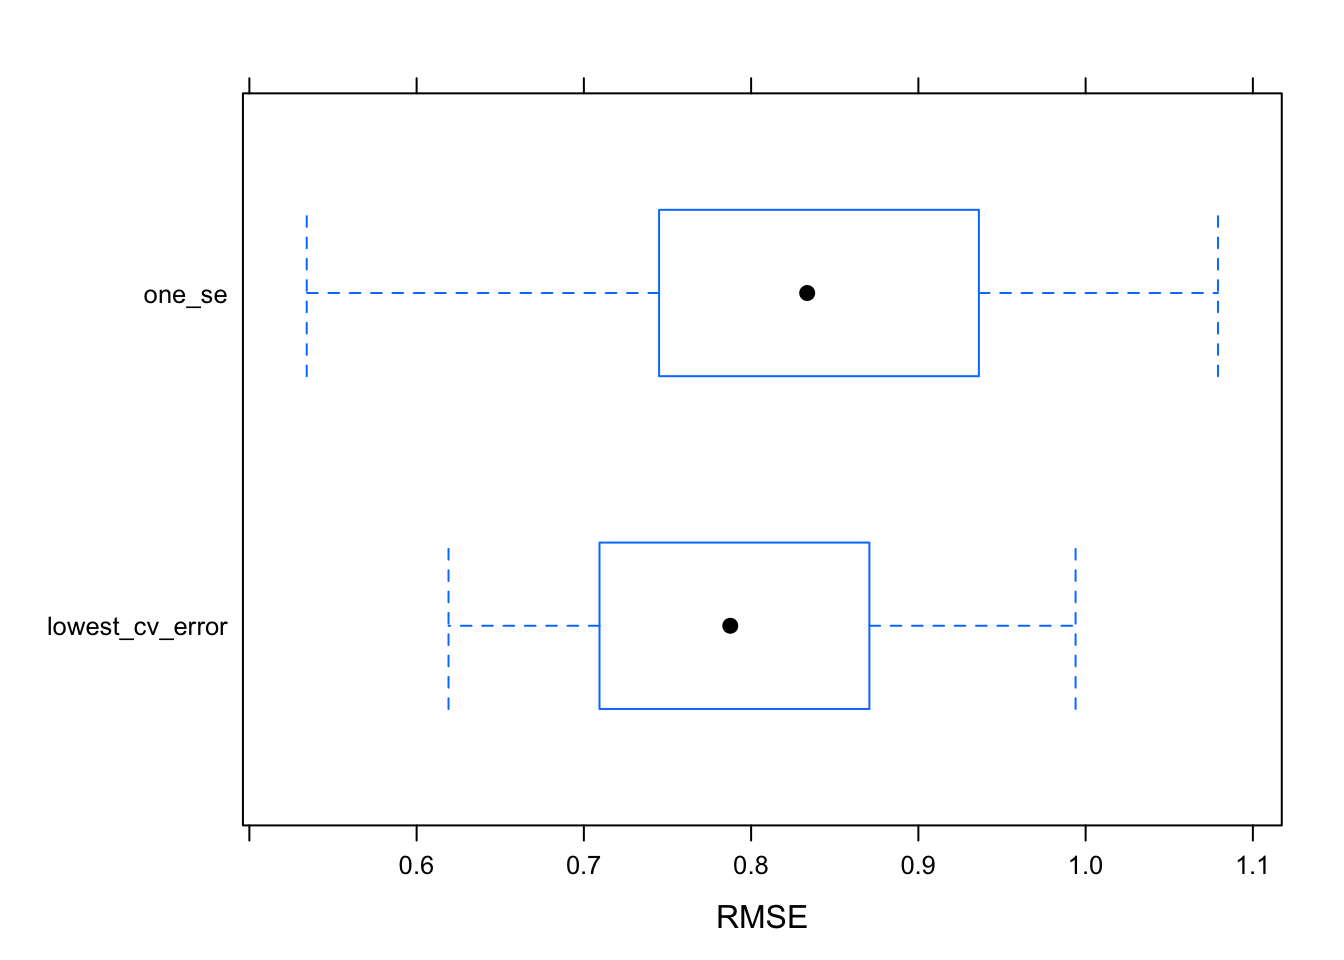
\includegraphics{hw4_files/figure-latex/unnamed-chunk-3-1.pdf}

\begin{Shaded}
\begin{Highlighting}[]
\NormalTok{tree\_fit\_2}\SpecialCharTok{$}\NormalTok{finalModel}\SpecialCharTok{$}\NormalTok{cptable}
\end{Highlighting}
\end{Shaded}

\begin{verbatim}
##           CP nsplit rel error
## 1 0.34710828      0 1.0000000
## 2 0.18464743      1 0.6528917
## 3 0.05931585      2 0.4682443
## 4 0.05247762      3 0.4089284
\end{verbatim}

\begin{Shaded}
\begin{Highlighting}[]
\FunctionTok{rpart.plot}\NormalTok{(tree\_fit\_2}\SpecialCharTok{$}\NormalTok{finalModel)}
\end{Highlighting}
\end{Shaded}

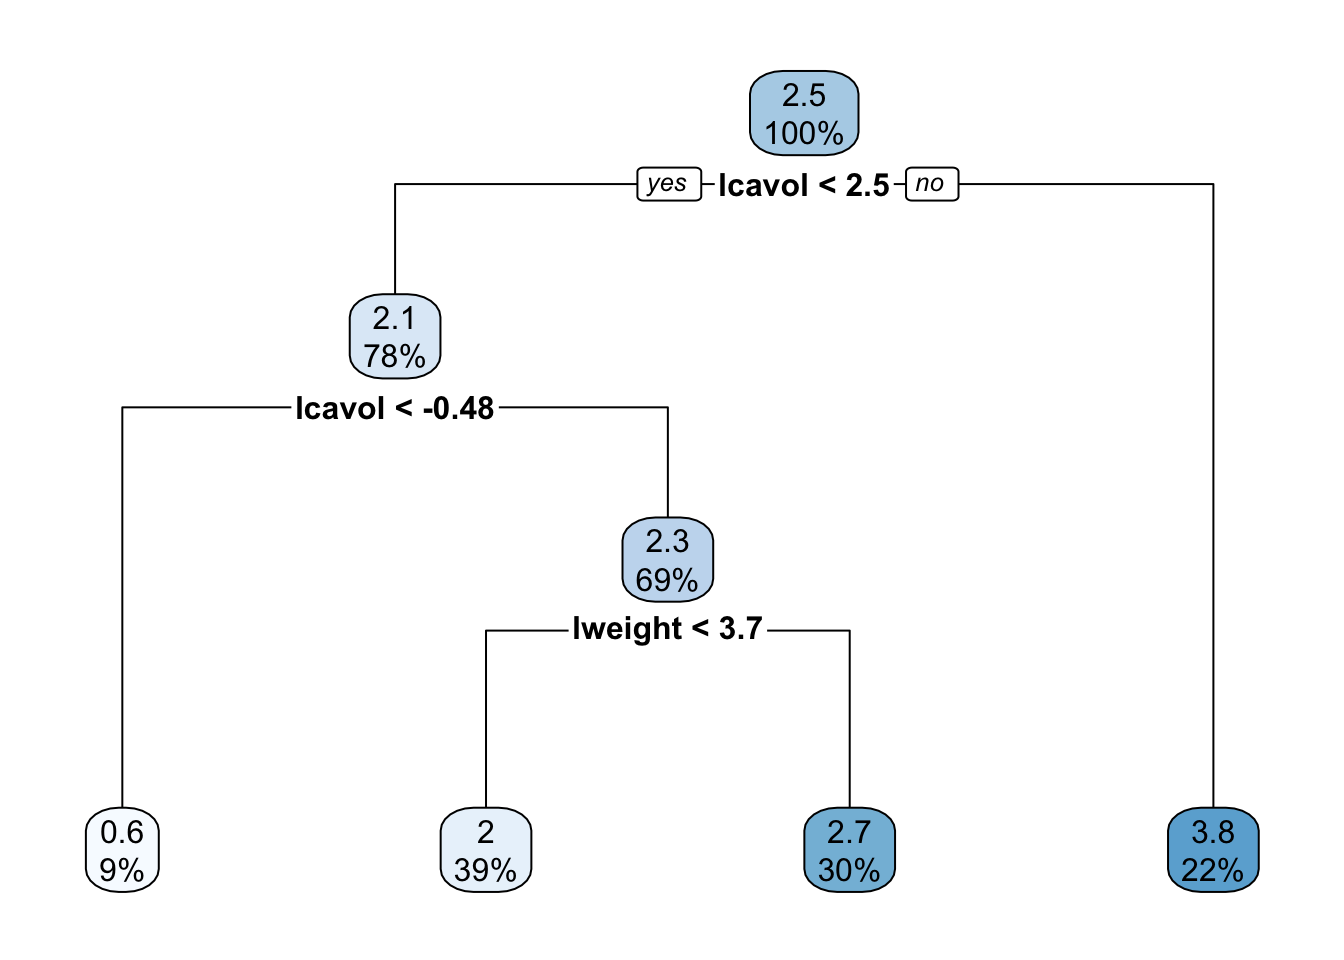
\includegraphics{hw4_files/figure-latex/unnamed-chunk-3-2.pdf}

The regression trees from lowest CV and 1 SE rule are different.

The tree corresponding to the lowest cross-validation error has a size
of 8, while the tree obtained with 1 SE rule has a size of 3

\hypertarget{b-choose-one-decision-tree-model}{%
\subsection{b) Choose one decision tree
model}\label{b-choose-one-decision-tree-model}}

\begin{Shaded}
\begin{Highlighting}[]
\NormalTok{resamp }\OtherTok{=} \FunctionTok{resamples}\NormalTok{(}\FunctionTok{list}\NormalTok{(}\AttributeTok{lowest\_cv\_error =}\NormalTok{ tree\_fit\_1, }
                         \AttributeTok{one\_se =}\NormalTok{ tree\_fit\_2}
\NormalTok{                         ))}
\FunctionTok{bwplot}\NormalTok{(resamp, }\AttributeTok{metric =} \StringTok{"RMSE"}\NormalTok{)}
\end{Highlighting}
\end{Shaded}

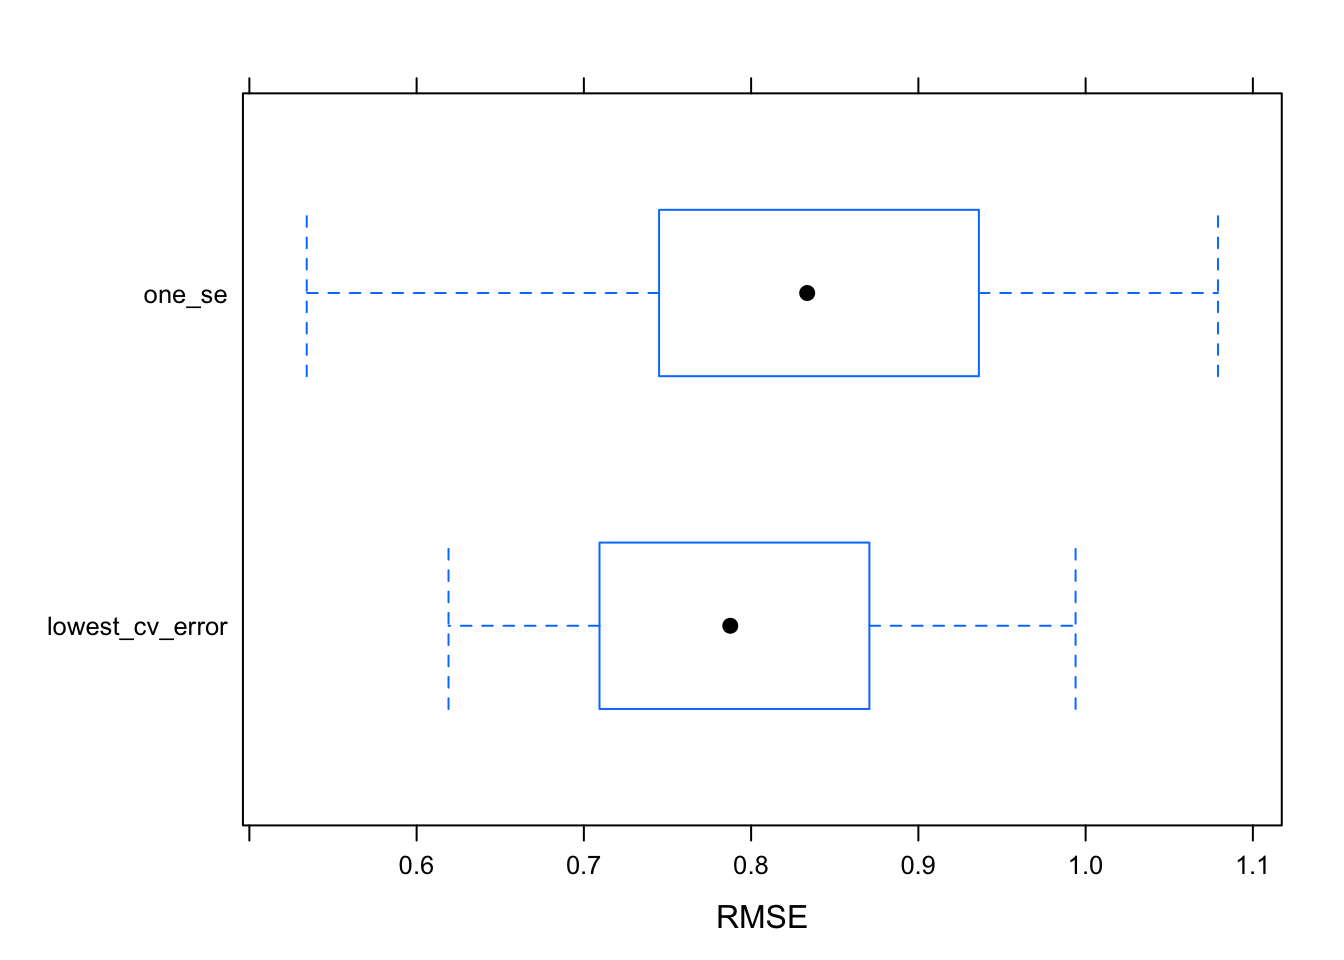
\includegraphics{hw4_files/figure-latex/unnamed-chunk-4-1.pdf}

I choosed tree size 3 as it has a similar performance with size 8 and it
is simpler.

\begin{Shaded}
\begin{Highlighting}[]
\FunctionTok{rpart.plot}\NormalTok{(tree\_fit\_2}\SpecialCharTok{$}\NormalTok{finalModel)}
\end{Highlighting}
\end{Shaded}

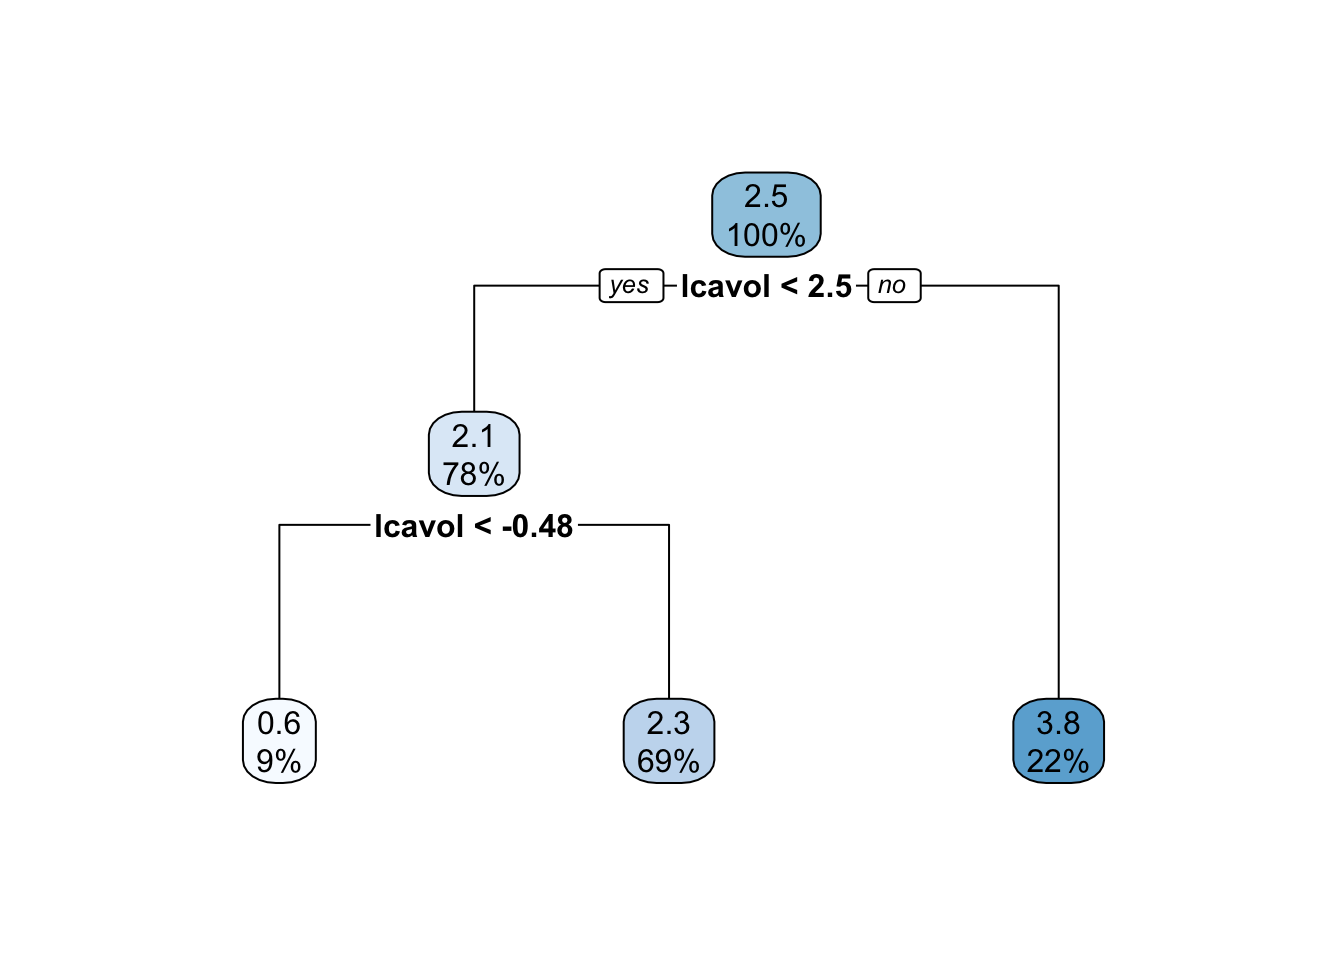
\includegraphics{hw4_files/figure-latex/unnamed-chunk-5-1.pdf}

The regression tree with size of 3 is chosen:

For the terminal node lcavol \textless{} 2.5, if log(cancer volumn) is
smaller than 2.5, there is 78\% of probability that log(prostate
specific antigen) to be 2.1. If lcovol is not smaller than 2.5, there is
22\% of probability that lpsa to be 3.8.

\hypertarget{c-bagging}{%
\subsection{c) Bagging}\label{c-bagging}}

\begin{Shaded}
\begin{Highlighting}[]
\FunctionTok{set.seed}\NormalTok{(}\DecValTok{1}\NormalTok{)}
\NormalTok{bagging.grid }\OtherTok{=} \FunctionTok{expand.grid}\NormalTok{(}\AttributeTok{mtry =} \DecValTok{8}\NormalTok{,}
                           \AttributeTok{splitrule =} \StringTok{"variance"}\NormalTok{,}
                           \AttributeTok{min.node.size =} \DecValTok{1}\SpecialCharTok{:}\DecValTok{30}\NormalTok{)}
\NormalTok{bag\_fit }\OtherTok{=} \FunctionTok{train}\NormalTok{(lpsa}\SpecialCharTok{\textasciitilde{}}\NormalTok{.,}
                \AttributeTok{data =}\NormalTok{ Prostate,}
                \AttributeTok{method =} \StringTok{"ranger"}\NormalTok{,}
                \AttributeTok{tuneGrid =}\NormalTok{ bagging.grid,}
                \AttributeTok{importance =} \StringTok{"impurity"}\NormalTok{,}
                \AttributeTok{trControl =} \FunctionTok{trainControl}\NormalTok{(}\AttributeTok{method =} \StringTok{"cv"}\NormalTok{))}

\FunctionTok{ggplot}\NormalTok{(bag\_fit, }\AttributeTok{highlight =} \ConstantTok{TRUE}\NormalTok{)}
\end{Highlighting}
\end{Shaded}

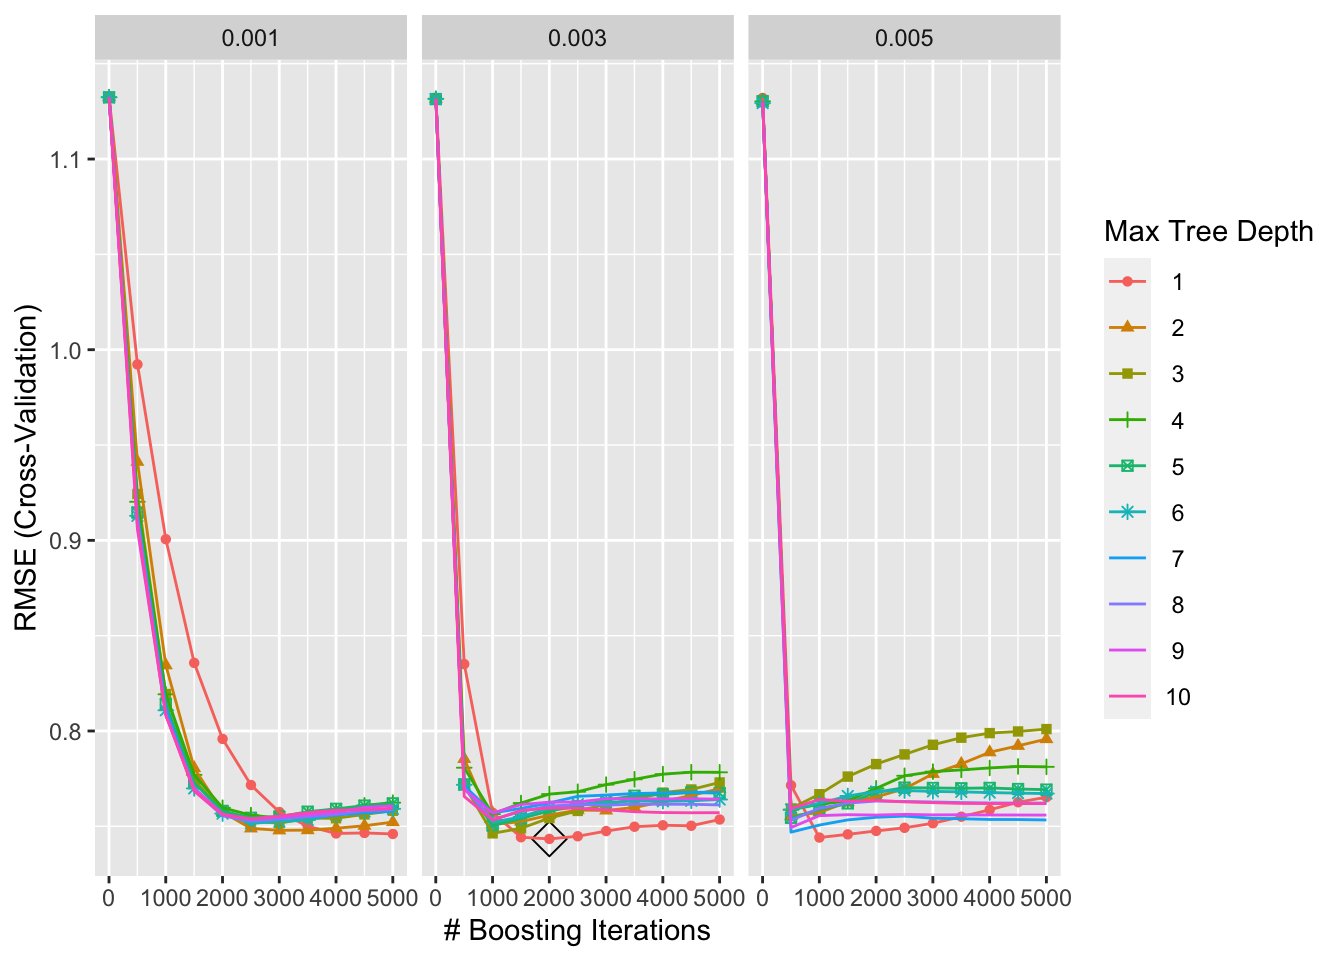
\includegraphics{hw4_files/figure-latex/unnamed-chunk-6-1.pdf}

\begin{Shaded}
\begin{Highlighting}[]
\FunctionTok{barplot}\NormalTok{(}\FunctionTok{sort}\NormalTok{(ranger}\SpecialCharTok{::}\FunctionTok{importance}\NormalTok{(bag\_fit}\SpecialCharTok{$}\NormalTok{finalModel), }\AttributeTok{decreasing =} \ConstantTok{FALSE}\NormalTok{),}
        \AttributeTok{las =} \DecValTok{2}\NormalTok{, }\AttributeTok{horiz =} \ConstantTok{TRUE}\NormalTok{, }\AttributeTok{cex.names =} \FloatTok{0.7}\NormalTok{,}
        \AttributeTok{col =} \FunctionTok{colorRampPalette}\NormalTok{(}\AttributeTok{colors =} \FunctionTok{c}\NormalTok{(}\StringTok{"darkred"}\NormalTok{,}\StringTok{"white"}\NormalTok{,}\StringTok{"darkblue"}\NormalTok{))(}\DecValTok{19}\NormalTok{))}
\end{Highlighting}
\end{Shaded}

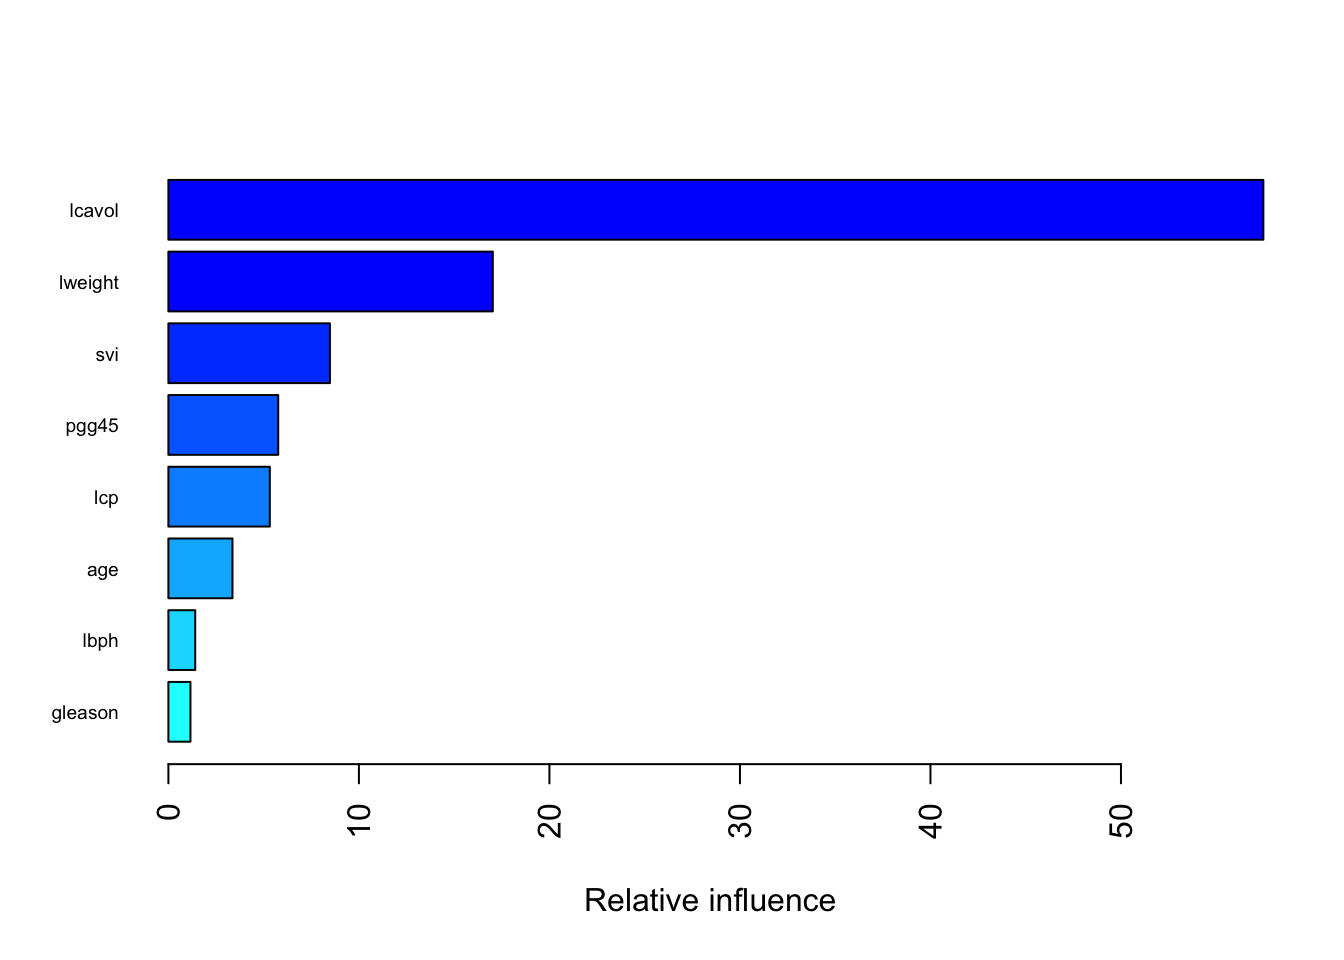
\includegraphics{hw4_files/figure-latex/unnamed-chunk-6-2.pdf}

Variable Importance: lcavol \textgreater{} lweight \textgreater{} svi
\textgreater{} pgg45 \textgreater{} lcp \textgreater{} age
\textgreater{} lbph \textgreater{} gleason

\hypertarget{d-random-forests}{%
\subsection{d) Random Forests}\label{d-random-forests}}

\begin{Shaded}
\begin{Highlighting}[]
\FunctionTok{set.seed}\NormalTok{(}\DecValTok{1}\NormalTok{)}
\NormalTok{rf.grid }\OtherTok{=} \FunctionTok{expand.grid}\NormalTok{(}\AttributeTok{mtry =} \DecValTok{1}\SpecialCharTok{:}\DecValTok{6}\NormalTok{, }\AttributeTok{splitrule =} \StringTok{"variance"}\NormalTok{, }\AttributeTok{min.node.size =} \DecValTok{1}\SpecialCharTok{:}\DecValTok{30}\NormalTok{)}

\NormalTok{rf\_fit }\OtherTok{=} \FunctionTok{train}\NormalTok{(lpsa}\SpecialCharTok{\textasciitilde{}}\NormalTok{.,}
               \AttributeTok{data =}\NormalTok{ Prostate,}
               \AttributeTok{method =} \StringTok{"ranger"}\NormalTok{,}
               \AttributeTok{tuneGrid =}\NormalTok{ rf.grid,}
               \AttributeTok{importance =} \StringTok{"impurity"}\NormalTok{,}
               \AttributeTok{trControl =} \FunctionTok{trainControl}\NormalTok{(}\AttributeTok{method =} \StringTok{"cv"}\NormalTok{))}

\FunctionTok{ggplot}\NormalTok{(rf\_fit, }\AttributeTok{highlight =} \ConstantTok{TRUE}\NormalTok{)}
\end{Highlighting}
\end{Shaded}

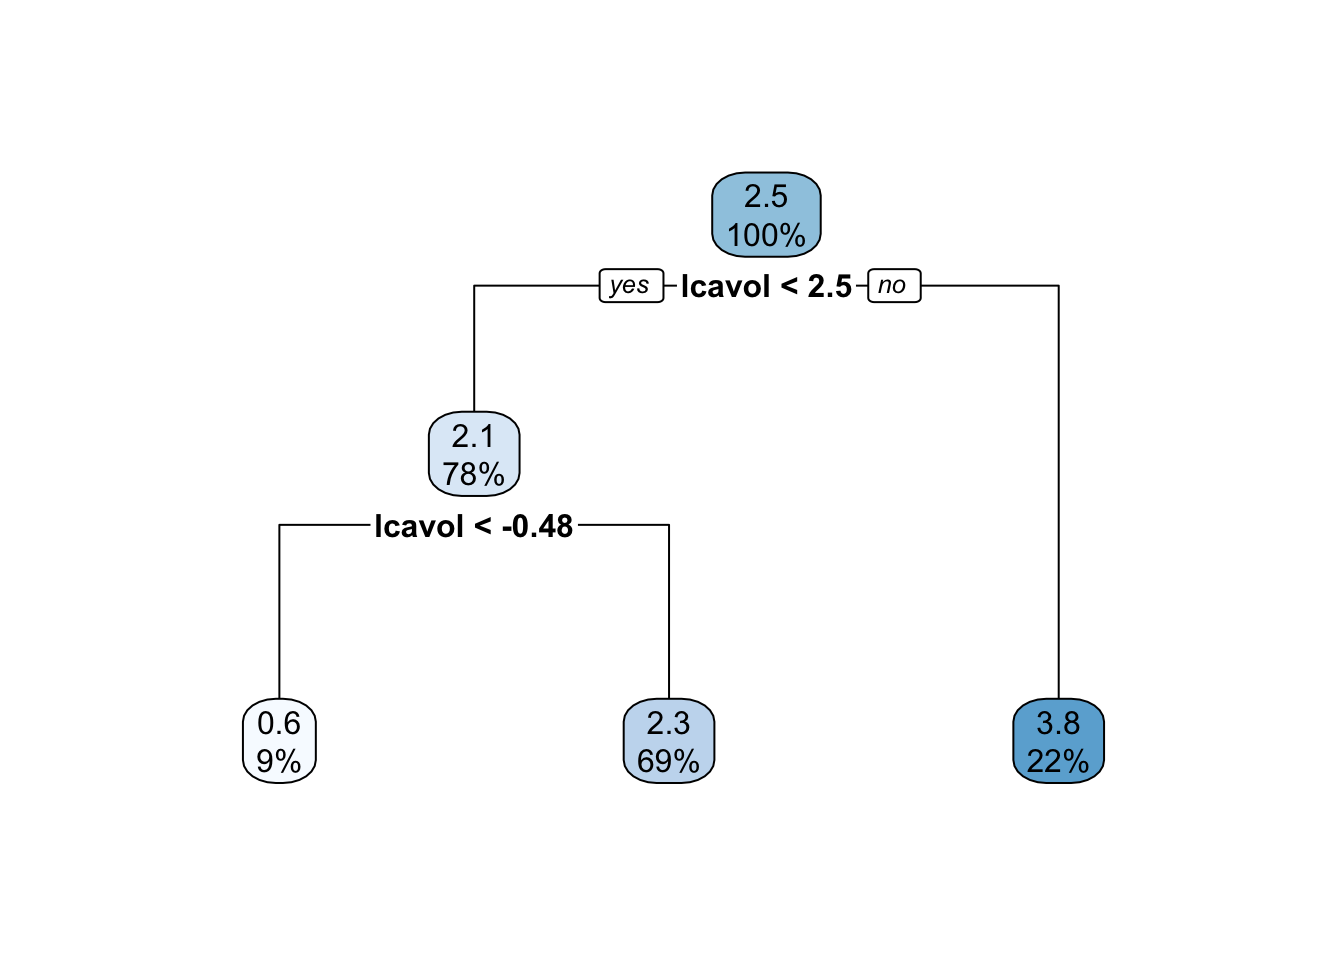
\includegraphics{hw4_files/figure-latex/unnamed-chunk-7-1.pdf}

\begin{Shaded}
\begin{Highlighting}[]
\FunctionTok{barplot}\NormalTok{(}\FunctionTok{sort}\NormalTok{(ranger}\SpecialCharTok{::}\FunctionTok{importance}\NormalTok{(rf\_fit}\SpecialCharTok{$}\NormalTok{finalModel), }\AttributeTok{decreasing =} \ConstantTok{FALSE}\NormalTok{),}
        \AttributeTok{las =} \DecValTok{2}\NormalTok{, }\AttributeTok{horiz =} \ConstantTok{TRUE}\NormalTok{, }\AttributeTok{cex.names =} \FloatTok{0.7}\NormalTok{,}
        \AttributeTok{col =} \FunctionTok{colorRampPalette}\NormalTok{(}\AttributeTok{colors =} \FunctionTok{c}\NormalTok{(}\StringTok{"darkred"}\NormalTok{,}\StringTok{"white"}\NormalTok{,}\StringTok{"darkblue"}\NormalTok{))(}\DecValTok{19}\NormalTok{))}
\end{Highlighting}
\end{Shaded}

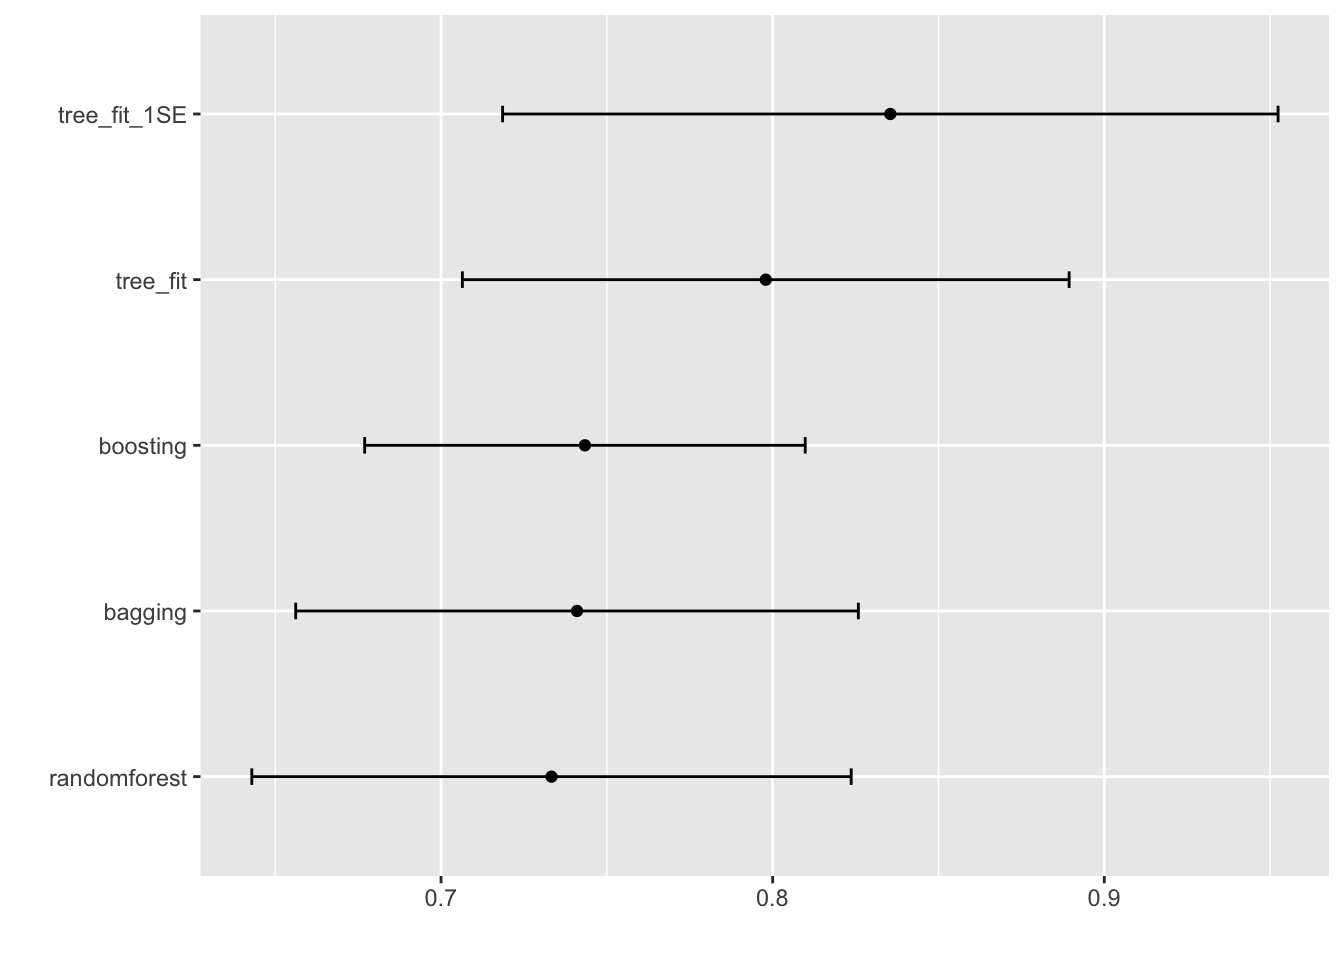
\includegraphics{hw4_files/figure-latex/unnamed-chunk-7-2.pdf}

Variable Importance: lcavol \textgreater{} lweight \textgreater{} svi
\textgreater{} lcp \textgreater{} pgg45 \textgreater{} age
\textgreater{} lbph \textgreater{} gleason

\hypertarget{e-boosting}{%
\subsection{e) Boosting}\label{e-boosting}}

\begin{Shaded}
\begin{Highlighting}[]
\FunctionTok{set.seed}\NormalTok{(}\DecValTok{1}\NormalTok{)}

\NormalTok{gbm.grid }\OtherTok{=} \FunctionTok{expand.grid}\NormalTok{(}\AttributeTok{n.trees =} \FunctionTok{seq}\NormalTok{(}\DecValTok{1}\NormalTok{,}\DecValTok{5001}\NormalTok{, }\AttributeTok{by =} \DecValTok{500}\NormalTok{),}
                       \AttributeTok{interaction.depth =} \DecValTok{1}\SpecialCharTok{:}\DecValTok{10}\NormalTok{,}
                       \AttributeTok{shrinkage =} \FunctionTok{c}\NormalTok{(}\FloatTok{0.001}\NormalTok{, }\FloatTok{0.003}\NormalTok{, }\FloatTok{0.005}\NormalTok{),}
                       \AttributeTok{n.minobsinnode =} \DecValTok{1}\NormalTok{)}

\NormalTok{gbm\_fit }\OtherTok{=} \FunctionTok{train}\NormalTok{(lpsa}\SpecialCharTok{\textasciitilde{}}\NormalTok{.,}
                \AttributeTok{data =}\NormalTok{ Prostate,}
                \AttributeTok{method =} \StringTok{"gbm"}\NormalTok{,}
                \AttributeTok{tuneGrid =}\NormalTok{ gbm.grid,}
                \AttributeTok{trControl =} \FunctionTok{trainControl}\NormalTok{(}\AttributeTok{method =} \StringTok{"cv"}\NormalTok{),}
                \AttributeTok{verbose =} \ConstantTok{FALSE}\NormalTok{)}
\end{Highlighting}
\end{Shaded}

\begin{verbatim}
## Warning in nominalTrainWorkflow(x = x, y = y, wts = weights, info = trainInfo, :
## There were missing values in resampled performance measures.
\end{verbatim}

\begin{Shaded}
\begin{Highlighting}[]
\FunctionTok{ggplot}\NormalTok{(gbm\_fit, }\AttributeTok{highlight =} \ConstantTok{TRUE}\NormalTok{)}
\end{Highlighting}
\end{Shaded}

\begin{verbatim}
## Warning: The shape palette can deal with a maximum of 6 discrete values because
## more than 6 becomes difficult to discriminate; you have 10. Consider
## specifying shapes manually if you must have them.
\end{verbatim}

\begin{verbatim}
## Warning: Removed 132 rows containing missing values (geom_point).
\end{verbatim}

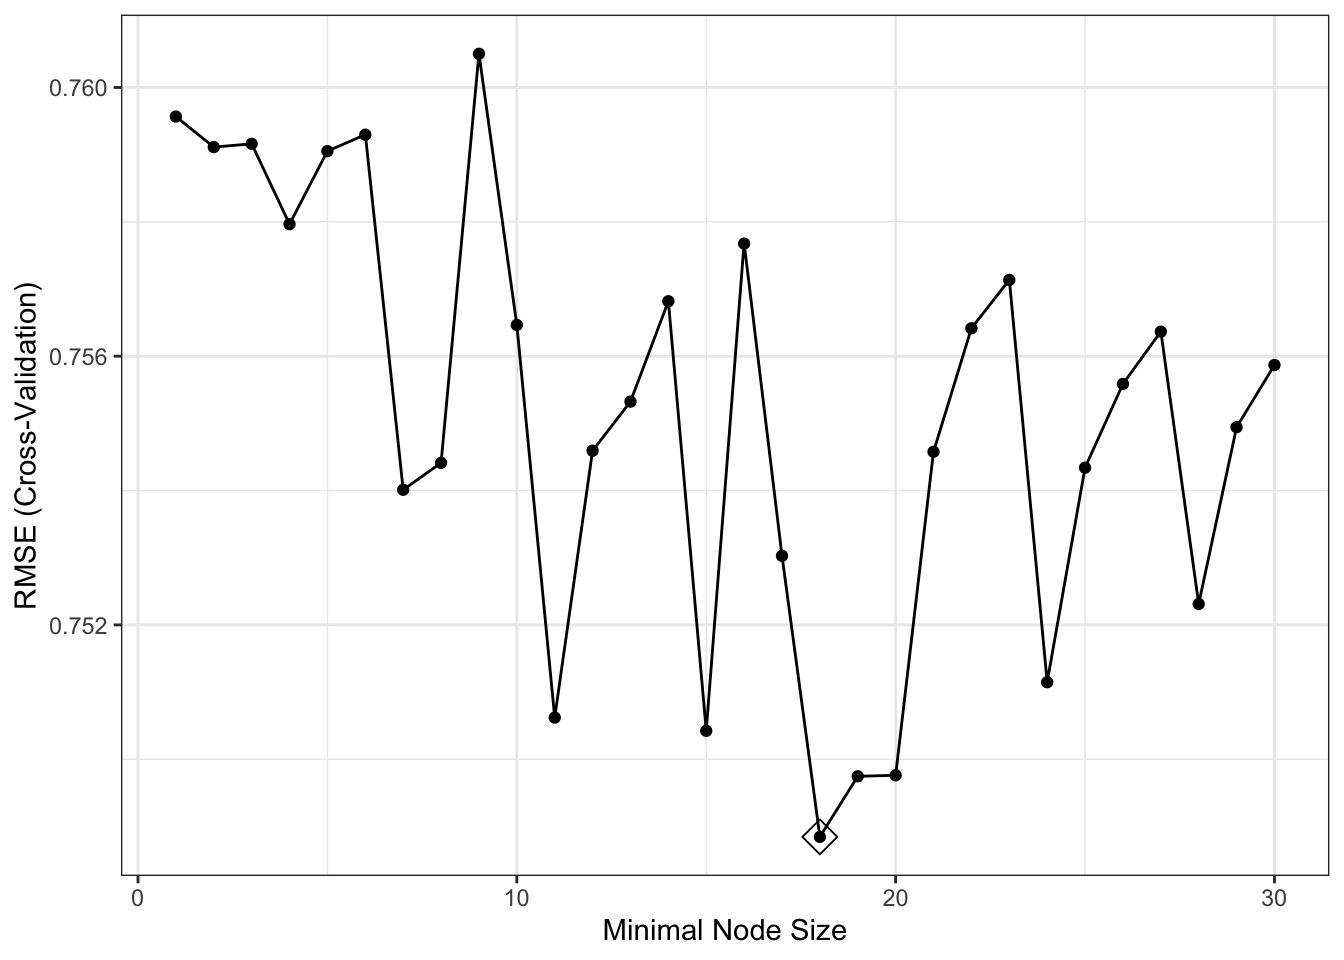
\includegraphics{hw4_files/figure-latex/unnamed-chunk-8-1.pdf}

\begin{Shaded}
\begin{Highlighting}[]
\FunctionTok{summary}\NormalTok{(gbm\_fit}\SpecialCharTok{$}\NormalTok{finalModel, }\AttributeTok{las =} \DecValTok{2}\NormalTok{, }\AttributeTok{cBars =} \DecValTok{19}\NormalTok{, }\AttributeTok{cex.names =} \FloatTok{0.6}\NormalTok{)}
\end{Highlighting}
\end{Shaded}

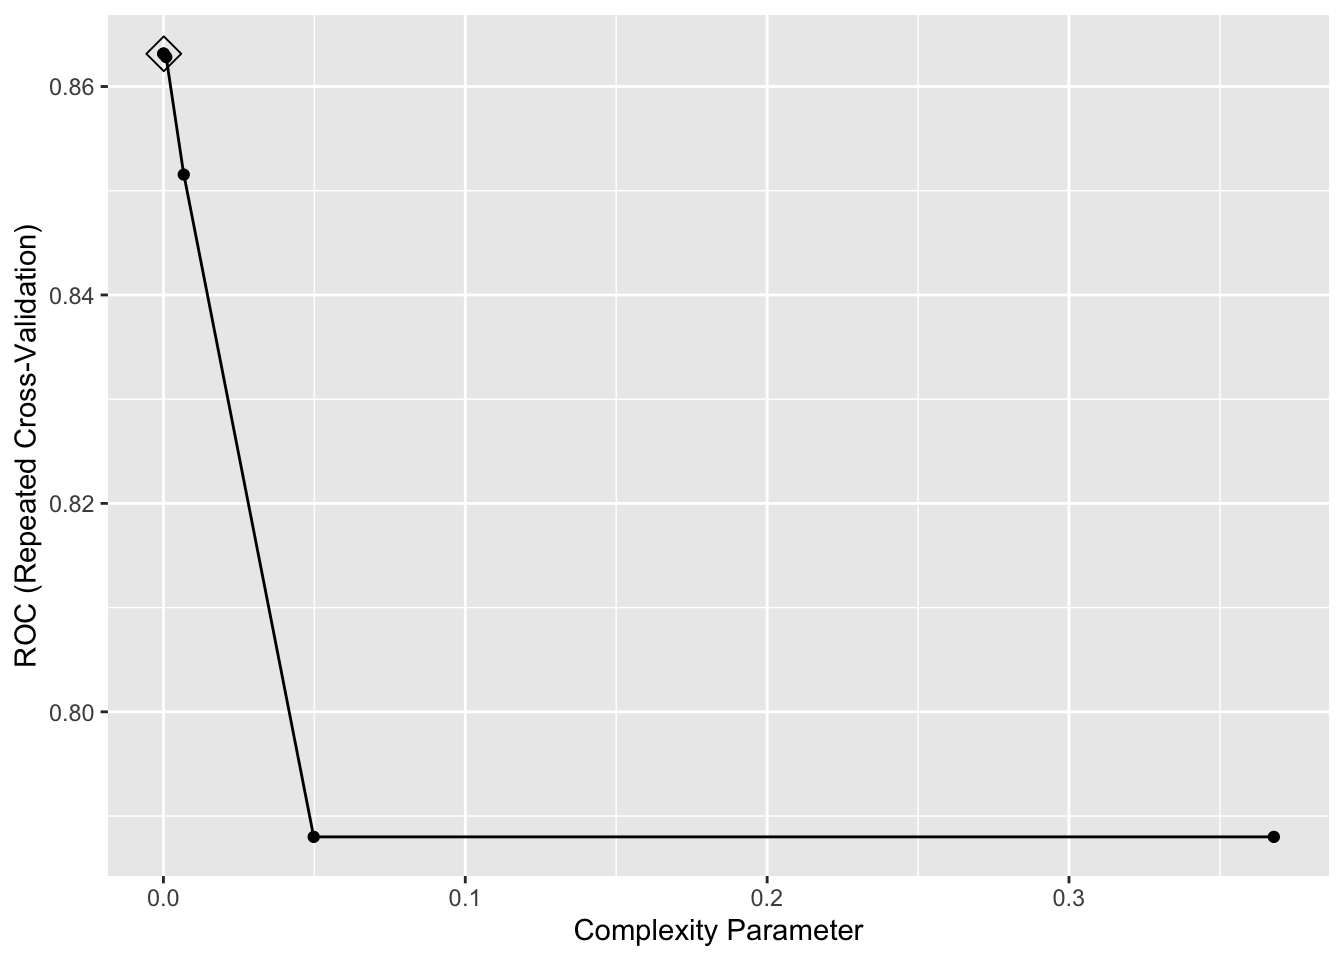
\includegraphics{hw4_files/figure-latex/unnamed-chunk-8-2.pdf}

\begin{verbatim}
##             var   rel.inf
## lcavol   lcavol 57.474056
## lweight lweight 17.027933
## svi         svi  8.479331
## pgg45     pgg45  5.765356
## lcp         lcp  5.323152
## age         age  3.363850
## lbph       lbph  1.407875
## gleason gleason  1.158447
\end{verbatim}

Variable Importance: lcavol \textgreater{} lweight \textgreater{} svi
\textgreater{} lcp \textgreater{} pgg45 \textgreater{} age
\textgreater{} lbph \textgreater{} gleason

\hypertarget{f-compare-models}{%
\subsection{f) Compare Models}\label{f-compare-models}}

\begin{Shaded}
\begin{Highlighting}[]
\NormalTok{resamp\_2 }\OtherTok{=} \FunctionTok{resamples}\NormalTok{(}\FunctionTok{list}\NormalTok{(}\AttributeTok{tree\_fit =}\NormalTok{ tree\_fit\_1, }
                          \AttributeTok{tree\_fit\_1SE =}\NormalTok{ tree\_fit\_2,}
                          \AttributeTok{bagging =}\NormalTok{ bag\_fit,}
                          \AttributeTok{randomforest =}\NormalTok{ rf\_fit,}
                          \AttributeTok{boosting =}\NormalTok{ gbm\_fit))}

\FunctionTok{summary}\NormalTok{(resamp\_2)}
\end{Highlighting}
\end{Shaded}

\begin{verbatim}
## 
## Call:
## summary.resamples(object = resamp_2)
## 
## Models: tree_fit, tree_fit_1SE, bagging, randomforest, boosting 
## Number of resamples: 10 
## 
## MAE 
##                   Min.   1st Qu.    Median      Mean   3rd Qu.      Max. NA's
## tree_fit     0.5293632 0.5729342 0.6481657 0.6633928 0.7207664 0.8777953    0
## tree_fit_1SE 0.4357075 0.5706012 0.7067185 0.6796373 0.7977977 0.8703550    0
## bagging      0.4433892 0.5506423 0.6187773 0.6028693 0.6563489 0.7295966    0
## randomforest 0.4554822 0.5436194 0.6180317 0.5994308 0.6636039 0.7080718    0
## boosting     0.4878801 0.5540710 0.6053314 0.6008631 0.6381473 0.6978078    0
## 
## RMSE 
##                   Min.   1st Qu.    Median      Mean   3rd Qu.      Max. NA's
## tree_fit     0.6190744 0.7169931 0.7875436 0.7979146 0.8638012 0.9939908    0
## tree_fit_1SE 0.5342864 0.7457950 0.8335274 0.8354868 0.9237662 1.0791335    0
## bagging      0.5332508 0.6602017 0.7460857 0.7410050 0.8218336 0.9104530    0
## randomforest 0.5435114 0.6387862 0.7393165 0.7333067 0.8108179 0.9294960    0
## boosting     0.5984236 0.6748127 0.7519523 0.7433897 0.7848678 0.9074745    0
## 
## Rsquared 
##                    Min.   1st Qu.    Median      Mean   3rd Qu.      Max. NA's
## tree_fit     0.11990318 0.3945387 0.5620070 0.5332883 0.7161215 0.7679649    0
## tree_fit_1SE 0.04643869 0.4688282 0.5393638 0.5061726 0.6050400 0.7639059    0
## bagging      0.41035904 0.5274679 0.6165821 0.6181705 0.7020880 0.7821978    0
## randomforest 0.37094854 0.5517331 0.6145224 0.6207200 0.7081548 0.7822906    0
## boosting     0.37405448 0.5056192 0.6369519 0.6223847 0.7392506 0.8362165    0
\end{verbatim}

\begin{Shaded}
\begin{Highlighting}[]
\FunctionTok{bwplot}\NormalTok{(resamp\_2, }\AttributeTok{metric =} \StringTok{"RMSE"}\NormalTok{)}
\end{Highlighting}
\end{Shaded}

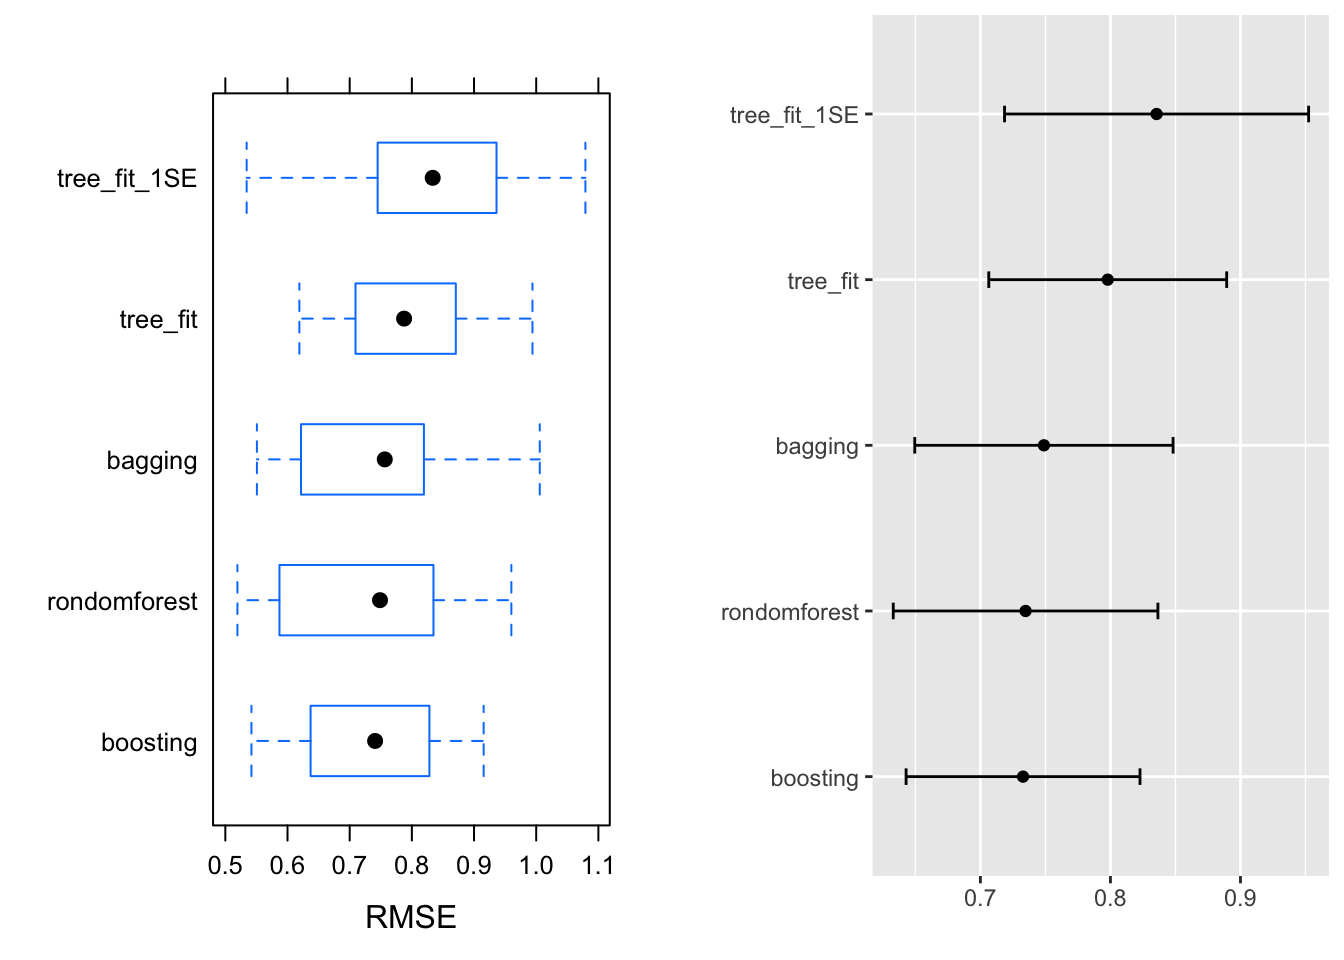
\includegraphics{hw4_files/figure-latex/unnamed-chunk-9-1.pdf}

\begin{Shaded}
\begin{Highlighting}[]
\FunctionTok{ggplot}\NormalTok{(resamp\_2, }\AttributeTok{metric =} \StringTok{"RMSE"}\NormalTok{)}
\end{Highlighting}
\end{Shaded}

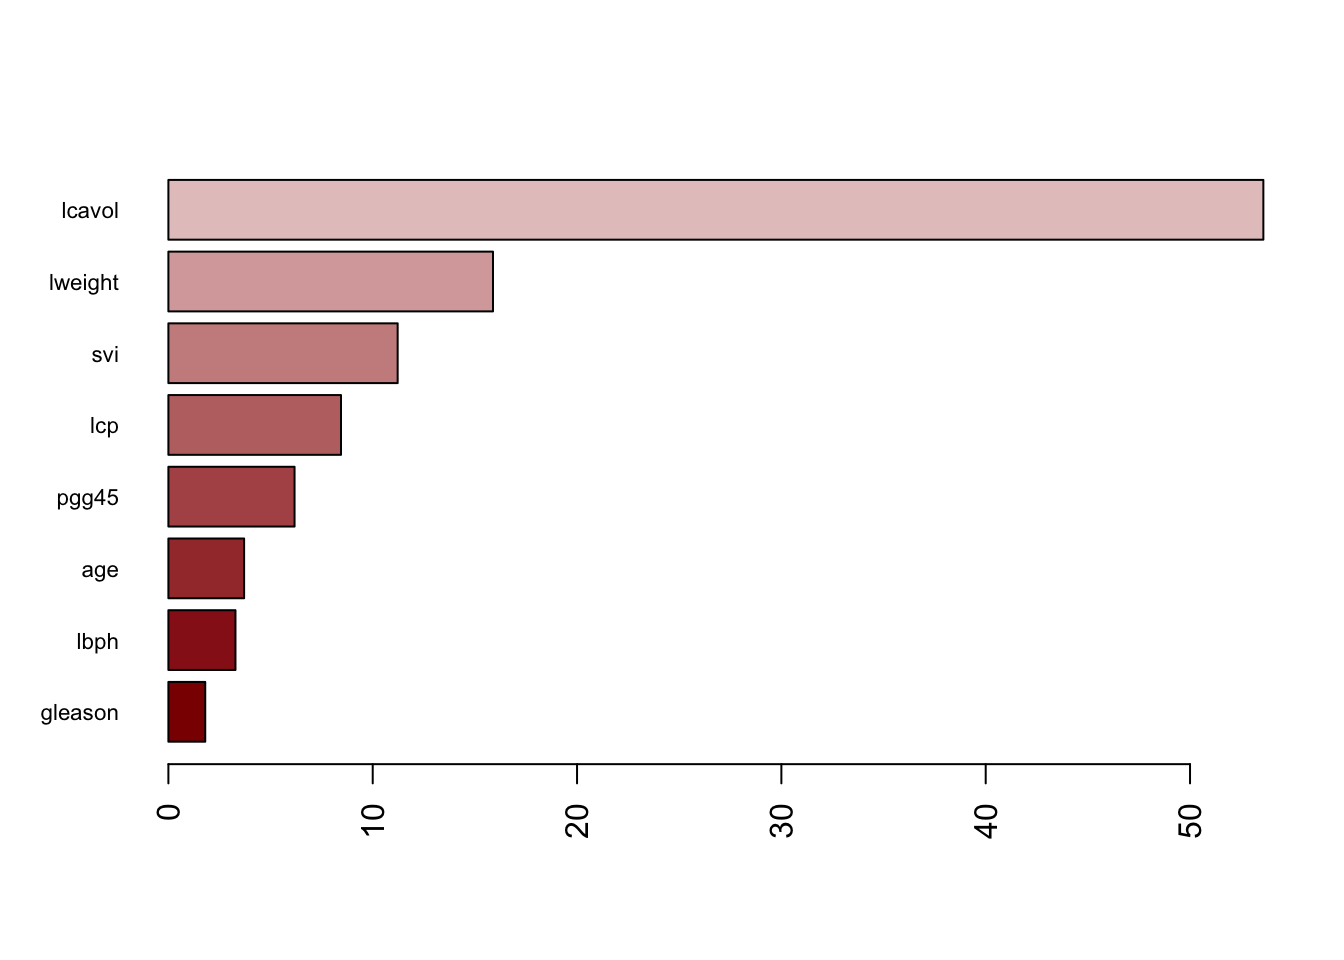
\includegraphics{hw4_files/figure-latex/unnamed-chunk-9-2.pdf}

Boosting, random forests and bagging have similar RMSE mean and median.
However, random forests has the largest mean R-squared value. Therefore,
random forests is chosen to predict PSA level.

\end{document}
